\section{ХОД РАБОТЫ}

\subsection{Постановка задачи}

Необходимо разработать программу на языке Ассемблер, 
которая выполняла бы следующую последовательность действий:

\begin{enumerate}
  \item считывание содержимого четырех текстовых файлов;
  \item запись в результирующий файл общее содержимое всех
    возможных троек, которые можно составить из четверки текстовых файлов.
\end{enumerate}

Схематично содержимое файла с результатом работы программы можно представить 
в виде кругов Эйлера, представленных на рисунке~\ref{pic:scheme}.
Разноцветные круги Эйлера соответствуют исходным файлам, а область, отмеченная
красным цветом --- результату работы программы.

\begin{figure}[h!]
  \centering
  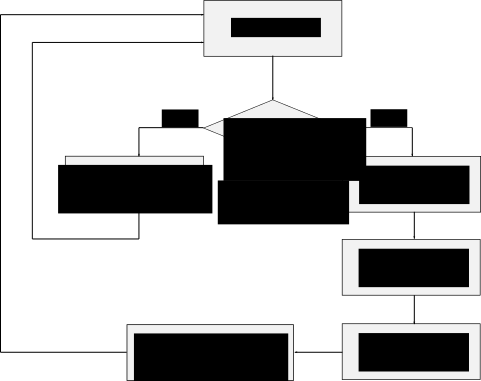
\includegraphics[width=0.8\linewidth]{pic/scheme}
  \caption{Представление результата работы программы \\ в виде кругов Эйлера}
  \label{pic:scheme}
\end{figure}

Программа должна быть написана с использованием цепочечных команд.
Допустимо установить ограничение на максимальный размер анализируемых файлов,
исходя из установленного размера буферов хранения цепочек.

\subsection{Особенности разработанной программы}

Программа написана с на основе макросов, разработанных в ходе
предыдущей лабораторной работы.

Центральная часть программы --- макрос, реализующий выделение
общей части двух цепочек, приведенный на рисунке~\ref{lst:macro_and}.

\begin{lstlisting}[caption=Макрос выделения общих значений двух цепочек,
label=lst:macro_and,language={[x86masm]Assembler},basicstyle=\scriptsize\ttfamily]
 BufAND   macro buffer_1,len_buffer_1, buffer_2,len_buffer_2, buffer_res,len_buffer_res, max_size
     local   _loop_,_next_,_store_,_end_       
 
     lea     bx, buffer_1
 
     mov     dx, 0               ; length of result
     cld
 _loop_:
     mov     al,[bx]
     lea     di, buffer_2
     mov     cx, len_buffer_2
     
     repne   scasb
     cmp     cx, 0    
     je      _next_
 
     ;; check, if buffer_tmp is empty
     cmp     dx, 0
     je      _store_
     ;; else check,
     ;; if this value already exists in buffer_tmp 
     lea     di, buffer_res
     mov     cx, dx              ; cx = dx + 1
     inc     cx
     repne   scasb
     cmp     cx, 0
     jg      _next_
 
 _store_:
     ;; if not, then store result        
     lea     di, buffer_res
     add     di, dx
     stosb
     inc     dx
 
 _next_: 
     inc     bx        
 
     ;; check if it's end of buffer_1
     mov     cx, bx
     sub     cx, offset buffer_1
     cmp     cx, len_buffer_1
     jl      _loop_
         
 _end_:
     mov     len_buffer_res, dx
     endm
\end{lstlisting}

Данный макрос выполняет попарное сравнение участков памяти, адресуемых опeрандами
buffer\_1 и buffer\_2 (с длиной значимой части len\_buffer\_1 и len\_buffer\_2 соответственно),
и заносит общую часть этих участков памяти в третий участок памяти,
адресуемый оператором buffer\_res.

Работа с файловой системой (создание, открытие, чтение, запись и закрытие файлов) осуществляется
с помощью семейства функций работы с файлам DOS, использующих файловые дескрипторы.

Пример работы программы показан на рисунке~\ref{lst:result}.

\begin{lstlisting}[caption=Пример работы программы,
label=lst:result,basicstyle=\scriptsize\ttfamily]
# source
C:\input\a.txt:
ABC

C:\input\b.txt:
BCD

C:\input\c.txt:
CDE

C:\input\d.txt:
DEF

# result
Warning: maximal sensible size of file is 512 bytes

C:\input\a.txt & C:\input\b.txt & C:\input\c.txt:
C

C:\input\b.txt & C:\input\c.txt & C:\input\d.txt:
D

C:\input\a.txt & C:\input\c.txt & C:\input\d.txt: # nothing

C:\input\a.txt & C:\input\b.txt & C:\input\d.txt: # nothing

\end{lstlisting}

Исходный текст разработанной программы находится в приложении~А.
